\chapter{Introduction to Cryptography}

\section{Introduction}
Cryptography refers to hidden writing. Its goal is to enable a secure communication between two users (Alice and Bob), and making it impossible for an eavesdropper to understand the information being exchanged.

\begin{figure}
	\centering
	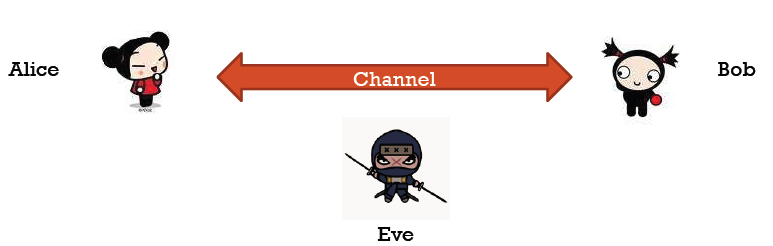
\includegraphics[width=0.7\linewidth]{Images/Chapter1/screenshot000}
	\caption{}
	\label{fig:chapter1_screenshot000}
\end{figure}

By channel we mean any physical or logical medium of communication from one user to another. A channel becomes secure when the information exchanged over it cannot be overheard or tampered with by eavesdroppers. By default a channel is considered insecure, so the intent of cryptography is to make secure, an insecure channel.

To transmit data in a secure way Alice and Bob rather than transmitting the message in a plain form they first covert it to a disguised form. Formally these are called plaintext ($\mathcal{P}$) and ciphertext ($\mathcal{C}$). The idea is to transform a plaintext into a ciphertext, so that Alice sends the latter to Bob, and Bob is able to reconstruct the plaintext from the received ciphertext while this is very difficult (almost impossible) for Eve.

In practice there is a pair of functions:
\begin{itemize}
	\item $enc: \mathcal{P \rightarrow C}$
	\item $dec: \mathcal{C \rightarrow P}$
\end{itemize}
Such that $dec(enc(m)) = m$ for every $m\in\mathcal{P}$.
For this to work Alice and Bob need to agree on what encryption and decryption scheme to use without disclosing it to Eve. Eve will only be able to observe ciphertexts, but notice that if the sets of plaintexts and ciphertexts are too small, then Eve can try all the plaintext-ciphertext pairs (exhaustive search) or even if the sets of plaintexts and ciphertexts are large enough to make exhaustive search impractical, encryption and decryption can be defined in obvious way to allow Eve to easily reconstruct them (guessing).
There is a problem with this formalization: these two functions, must be kept secret. These function can be used to create a secure channel, but how do you share these function? We need a secure channel, but if we had a secure channel, why not use it in the first place?

Since otherwise we would have to define and encryption and decryption functions for each pair of people that want to communicate securely we introduce the concept of a cryptographic key. We denote the set of (cryptographic) keys with $\mathcal{K}$, and consider a map 
$\varphi : \mathcal{P} \times \mathcal{K} \rightarrow \mathcal{C}$ such that for every key $k\in \mathcal{K}$ the function $\varphi(\cdot, k) : \mathcal{P} \rightarrow \mathcal{C}$ is an encryption function.

There are some key differences with respect to the old functions:
\begin{itemize}
	\item The definition of $\varphi$ (encryption algorithm) can be very complex but it can be public(i.e. known to anyone) and Alice and Bob can agree on it over an insecure channel. Before the encryption algorithm had to be private.
	\item The only component that must be kept secret(and thus exchanged over a secure channel) is the cryptographic key $k$, that defines the encryption function to use
\end{itemize}

The Kerchkhoff principle states that a cryptosystem should be secure even if everything about the system, except the key, is public knowledge. The advantages to only exchanging cryptographic keys rather than ciphers are that it is easier to keep secret $k$ than $\varphi$, and if the key is discovered it is sufficient to choose another key. The main disadvantage is that the attacker only needs to find the key to break the system.


\section{Attacks}
Let’s now consider some useful attack models expressed in terms of what the attacker can observe and what queries they can make to the cipher. A query for our purposes is the operation that sends an input value to some function and gets the output in return, without exposing the details of that function. An encryption query, for example, takes a plaintext and returns a corresponding ciphertext, without revealing the secret key. We call these models black-box models, because the attacker only sees what goes in and out of the cipher.
There are several different black-box attack models.  Note that the higher the attacker skills and complexity of the attack the less (computational) effort the attacker needs to put to break the system.

	\subsection{Ciphertext-only attackers (COA)}
	Ciphertext-only attackers (COA), or known-ciphertext attackers, observe ciphertexts but don’t know the 	associated plaintexts, and don’t know how the plaintexts were selected. Attackers in the COA model are passive and can’t perform encryption or decryption queries. The task of the attacker is very difficult and a lot of computational power is required to mount such an attack, this is because the attacker needs to check for every possibile key of if the decrypted ciphertext is meaningful \ref{fig:coa}.
	\begin{figure}
		\centering
		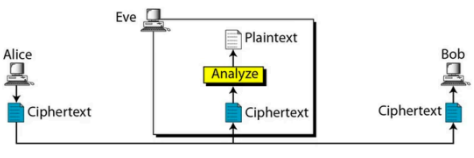
\includegraphics[width=0.7\linewidth]{Images/Chapter1/coa}
		\caption{}
		\label{fig:coa}
	\end{figure}
	
	In some cases the attacker only needs to know the probability distribution of the plaintexts, it could obtain a lot of information merely by observing some ciphertexts. This holds under the assumption that all plaintexts are encrypted with the same cipher and the same key. The method may be difficult (if possible at all) to apply to short messages or messages that contain words with many occurrences of letters with low frequencies. More information can be found \href{https://crypto.interactive-maths.com/frequency-analysis-breaking-the-code.html}{here}.


	\subsection{Known-plaintext attackers (KPA)}
	Known-plaintext attackers (KPA) observe ciphertexts and do know the associated plaintexts. Attackers in the KPA model thus get a list of plaintext–ciphertext pairs, where plaintexts are assumed to be randomly selected. Again, KPA is a passive attacker model, thus the attacker can not choose a plaintext to encrypt.
	\begin{figure}
		\centering
		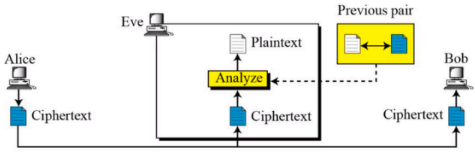
\includegraphics[width=0.7\linewidth]{Images/Chapter1/kpa}
		\caption{}
		\label{fig:kpa}
	\end{figure}
	
	Essentialy the attacker will attempt to do what is known as a key recovery attack. But recovering the key might be a difficult problem to solve, so Eve might try to discover a functionally equivalent algorithm for encryption and decryption, or else design cryptographic algorithm that, even without knowing the key $k$, produces the same result as those of the cipher with the key $k$. This kind of attacks are known as Global Deduction/Reconstruction attacks \ref{fig:kpa}.
	
	\subsection{Chosen-plaintext attackers (CPA)}
	Chosen-plaintext attackers (CPA) can perform encryption queries for	plaintexts of their choice and observe the resulting ciphertexts. This model captures situations where attackers can choose all or part of the plaintexts that are encrypted and then get to see the ciphertexts.
	Unlike COA or KPA, which are passive models, CPA are active attackers, because they influence the encryption processes rather than passively eavesdropping \ref{fig:cpa}.
	
	\begin{figure}
		\centering
		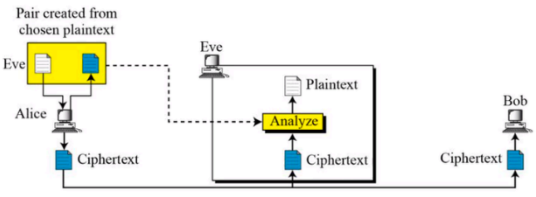
\includegraphics[width=0.7\linewidth]{Images/Chapter1/cpa}
		\caption{}
		\label{fig:cpa}
	\end{figure}
	
	With this the attacker may try to guess previously unknown plaintext-ciphertext pairs.
	
	
	\subsection{Chosen-ciphertext attackers (CCA)}
	Chosen-ciphertext attackers (CCA) \footnote{Not in the slides, maybe not required to know this} can both encrypt and decrypt; that is, they get to perform encryption queries and decryption queries. The CCA model may sound ludicrous at first—if you can decrypt, what else do you need?—but like the CPA model, it aims to represent situations where attackers can have some influence on the ciphertext and later get access to the plaintext. Moreover, decrypting something is not always enough to break a system.
	

\section{Shannon Theorem}

A cipher is broken if a method of determining the plaintext from the ciphertext is found without being legitimately given the decryption key. Any cryptosystem can be broken by an exhaustive key search. There exist ciphers that cannot be broken that are called perfect, and even exhaustive key search is of limited use for these ciphers.
A cipher is perfect if, after seeing the ciphertext, an attacker gets no extra information about the plaintext other than what was known before the ciphertext was observed. The attacker might know the kind of content hidden but not the content itself, the point is that the knowledge of the attacker about the plaintext is not increased after intercepting the ciphertext.
Let:
\begin{itemize}
	\item $\mathcal{K}$ be the set of keys
	\item $\mathcal{M}$ be the set of messages
	\item $\mathcal{C}$ be the set of ciphertexts
	\item $\varphi$ is a cipher such that $\forall k \in \mathcal{K}$
\end{itemize} 

$$\varphi_k : \mathcal{P} \rightarrow \mathcal{C}$$ is an encryption function.
Furthermore $\varphi_k$ is invertible: there exists $\varphi_k ^{-1}(\varphi_k(m)) = m$.
We will give a notion of probabilities:
\begin{itemize}
	\item if $m \in \mathcal{P}$, we use $P(m)$ to indicate the a priori probability that $m$ occurs.
	\item if $k \in \mathcal{K}$, $P(k)$, indicates the probability that k is the chosen key
	\item if $c \in \mathcal{C}$, $P(c)$ is the probability that $c$ is the transmitted ciphertext
	\item $P(\mathcal{P})$ is the probability distribution of the plaintexts
	\item $P(\mathcal{C})$ is the probability distribution of the ciphertexts
	\item $P(\mathcal{K})$ is the probability distribution of the keys
\end{itemize}
We can assume $P(m) > 0$ because otherwise $m$ never occurs and we can remove it from $\mathcal{P}$. In the same way we assume $P(k) > 0$ and $P(c) > 0$. The two probability distribution $P(\mathcal{P})$ and $P(\mathcal{K})$ determine the
probability distribution $P(\mathcal{C})$, because only one ciphertext can be obtained using the encryption algorithm $\varphi$ with a given plaintext and key.
Clever boy assumption states that plaintext and the keys are indipendent. So we do not select a particular key for a particular plaintext, for any plaintext we can choose any key. A cipher is called perfect if:
$$\forall m \in\mathcal{P} \land \forall c \in\mathcal{C} \Longrightarrow P(m) = P(m \mid c) $$
So the probability of having the plaintext $m$ is equal to the conditional probability of observing $m$ over the channel once you have seen the ciphertext $c$. The conditional probability $P(x \mid y)$ denotes the probability that $x$ occurs given that $y$ occurred. We say that $x$ and $y$ are independent if $P(x \land y) = P(x)P(y)$. The concept of independence formalises the perception that past events do not influence the outcome of future ones or provide any information about them. In other words, if two events are independent, the order in which they occur is of no importance. So seeing the ciphertext $c$ does not add any knowledge about the plaintext message sent, or any future message exchanged.

Shannon theorem: let us fix an integer $n$. Assume that: keys, plaintext, ciphertext have all $n$ bits. Assume also that the plaintexts and the keys are independent (Clever boy assumption) and any $n$-bit string may be either a key or a plaintext. Then $\varphi$ is a perfect cipher if and only if both the following conditions hold:
\begin{enumerate}
	\item the keys are perfectly random
	\item for any pair $(m,c)$ of plaintext-ciphertexts, there is one and only one key $k$ such that $c = \varphi(m,k)$
\end{enumerate}

	\subsection{Consequences of Shannon Theorem}
	
	If $\varphi$ is a perfect cipher, then all ciphertexts have the same probability to be received. Even if Eve knows the probability distribution of the plaintexts, she observes is a perfectly random cipher. Hence Eve cannot recover any information on the sent message from the intercepted ciphertext. But we made a very big assumption: this is true only if Eve can intercept \textbf{one} ciphertext. If Eve intercepts more ciphertexts encrypted with the same key, then the Shannon theorem no longer guarantees perfect secrecy. So in practical sense, a perfect cipher is not unbreakable, so a perfect cipher is not necessarily ideal, because every time we need to use a different key (the key space has to be as large as the message space) also the key has to be as large as a message transferred. Additionally we did not guarantee any sort of integrity! 

\section{Vernam Cipher - One Time Pad}

The One Time Pad is an example of a perfect cipher. We work under the same assumptions of the Shannon Theorem. In the Vernam cipher we define encryption by means of the bitwise XOR operation \ref{fig:vernam_cipher}:
$$c = \varphi_k (m) = k \oplus m$$

\begin{figure}
	\centering
	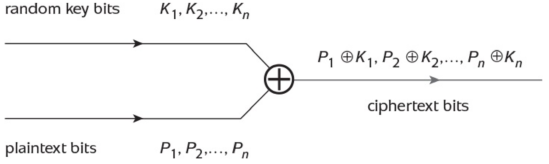
\includegraphics[width=0.7\linewidth]{Images/Chapter1/vernam_cipher}
	\caption{}
	\label{fig:vernam_cipher}
\end{figure}

Only if the key used is randomly chosen, this cipher is perfect.
But there are a few problems: how do we choose the key randomly, how is the key shared, and the fact length of the key used that has to be as long as the message shared (the storage needed doubles) and having to use a key just once. Let's say that Eve known a single plaintext-ciphertext pair ($m_1$,$c_1$), the key can be easily recovered as $m_1 \oplus c_1=m_1 \oplus (m_1 \oplus k)=(m_1 \oplus m_1) \oplus k= 0 \oplus k = k$. So any further messages exchanged with this key can be recovered by the attacker.

\section{From perfect to ideal}
We want the ability to encrypt a long message (e.g. a file of several megabytes) using a short key (e.g. a few hundred bits). We do not consider all possible adversaries, but only computationally feasible adversaries, that is, "real world" adversaries that must perform their calculations on real computers using a reasonable amount of time and memory. This leads to a weaker definition of security called semantic security. Furthermore, for our purposes a cipher is to be considered secure long as they do not leak any useful information about an encrypted message to an adversary other than the length of the message. Since the focus is on the "practical", instead of the "mathematically possible", one shall also insist that the encryption and decryption functions are themselves efficient algorithms and not just arbitrary functions.
So we'll study ciphers are regarded as secure in practice because the known theoretical attacks take too much time to conduct. In other words, to implement such theoretical attacks requires resources which are unrealistic for any attacker.

	\subsection{Practical secure ciphers}
	Characterizing the notion of practical security is not an easy task as it must consider several different aspects including:
	\begin{itemize}
		\item Cover time: the time window in which a plaintext must be kept secret. This suggests that no attack on the cipher can be conducted in less than the cover time and implies that an exhaustive key search takes longer than the cover time. Evaluation should be repeated if a new attack is discovered or other parameters are changed such as the available computation power.
		\item Computational complexity: what computational processes are involved in known attacks on the cryptosystem how much time it takes to conduct these processes. measuring the time taken to perform the processes requires a way of measuring the time it takes to run a process, or a function and this is expressed as a function of the size of the input that expresses the number of elementary operations performed, known as the Big O notation.
	\end{itemize}
	Most modern ciphers are regarded as secure in practice because the known theoretical attacks take too much time to conduct.
	Exhaustive key search has complexity $2^{n}$, assuming a computer can attempt a million keys per second, an exhaustive search in a 30-bit key space will be covered in about a thousand seconds.
	Establishing the complexity of any known attacks is important and useful, but brings no guarantees of practical security and this is because there are undiscovered theoretical attacks, problems with the implementation, key management issues and so on.
	How can we be sure an attacker will require a large amount of work to break a non-perfect system with every method? An alternative, it is to show that breaking the cipher can be reconducted to a computationally difficult problem. This is typically the approach used to show the security of public key ciphers.